\documentclass[10pt]{beamer}

\usepackage{amssymb,amsthm}% http://ctan.org/pkg/amssymb
\newtheorem{proposition}{Proposition}
\setbeamertemplate{theorems}[numbered]
\usecolortheme[RGB={100,0,0}]{structure}
\setbeamercolor{block title}{use=structure,fg=white,bg=structure.fg!75!black}
\setbeamercolor{block body}{parent=normal text,use=block title,bg=block title.bg!10!bg}

\usepackage{amsmath}
\DeclareMathOperator*{\argmax}{argmax}
\DeclareMathOperator*{\argmin}{argmin}

\usepackage{natbib}
\bibliographystyle{aea}

\usepackage{xcolor}
\usepackage{graphicx}
\usepackage{amsmath}
\usepackage{numprint}
\npdecimalsign{.}
\nprounddigits{3}
\usepackage{colortbl}
\usepackage{appendixnumberbeamer}
\usepackage{subfigure}
\usepackage{comment}

%\usepackage[hyperref]{beamerarticle} or 
\usepackage{hyperref}
\usepackage{caption}
%\captionsetup{font=scriptsize,labelfont=scriptsize}
\setbeamerfont{caption}{size=\scriptsize}
\usetheme{Singapore}
\usecolortheme{beaver}

% for adding regression tables
\usepackage{dcolumn} 
% column to line up decimals
\usepackage{booktabs,caption}
\captionsetup[table]{name=Table} 
\usepackage[flushleft]{threeparttable} 
% The above two allow that last line with the dagger as a bottom note.
\captionsetup{skip=0pt}

\usepackage{xcolor}
\definecolor{underbrace}{RGB}{30,199,166}
\newcommand{\textfrac}[1]{
  \begin{tabular}{@{}l@{}}#1\end{tabular}
}

\begin{document}

\title{Global Monetary Policy Shocks, Financial Frictions and Export Prices}
\author[Yao Amber LI, Lingfei LU and Jingbo YAO]{Yao Amber LI, Lingfei LU, Jingbo YAO}
\institute{\small HKUST}
\date{Dec 1, 2023}
\logo{
\includegraphics[scale=0.15]{UST4C_L3.eps}}

\begin{frame}
\maketitle
\centering
HKUST Research Postgraduate Student Workshop
\end{frame}

\AtBeginSection[]
{
    \begin{frame}{Outline}
    \transfade
    \tableofcontents[sectionstyle=show/shaded,subsectionstyle=show/shaded/hide]
    \addtocounter{framenumber}{-1}
    \end{frame}
}

%%%%%%%%%%%%%%%%%%%%%%%%%%%%%%%%%%%%%%%%%%%%%%%%%%%%%%
%%%%%%%%%%%%%%%%%%%%%%%%%%%%%%%%%%%%%%%%%%%%%%%%%%%%%%
\section{I. Introduction}

\begin{frame}{Motivation}
    \begin{figure}[htbp]
	\centering
	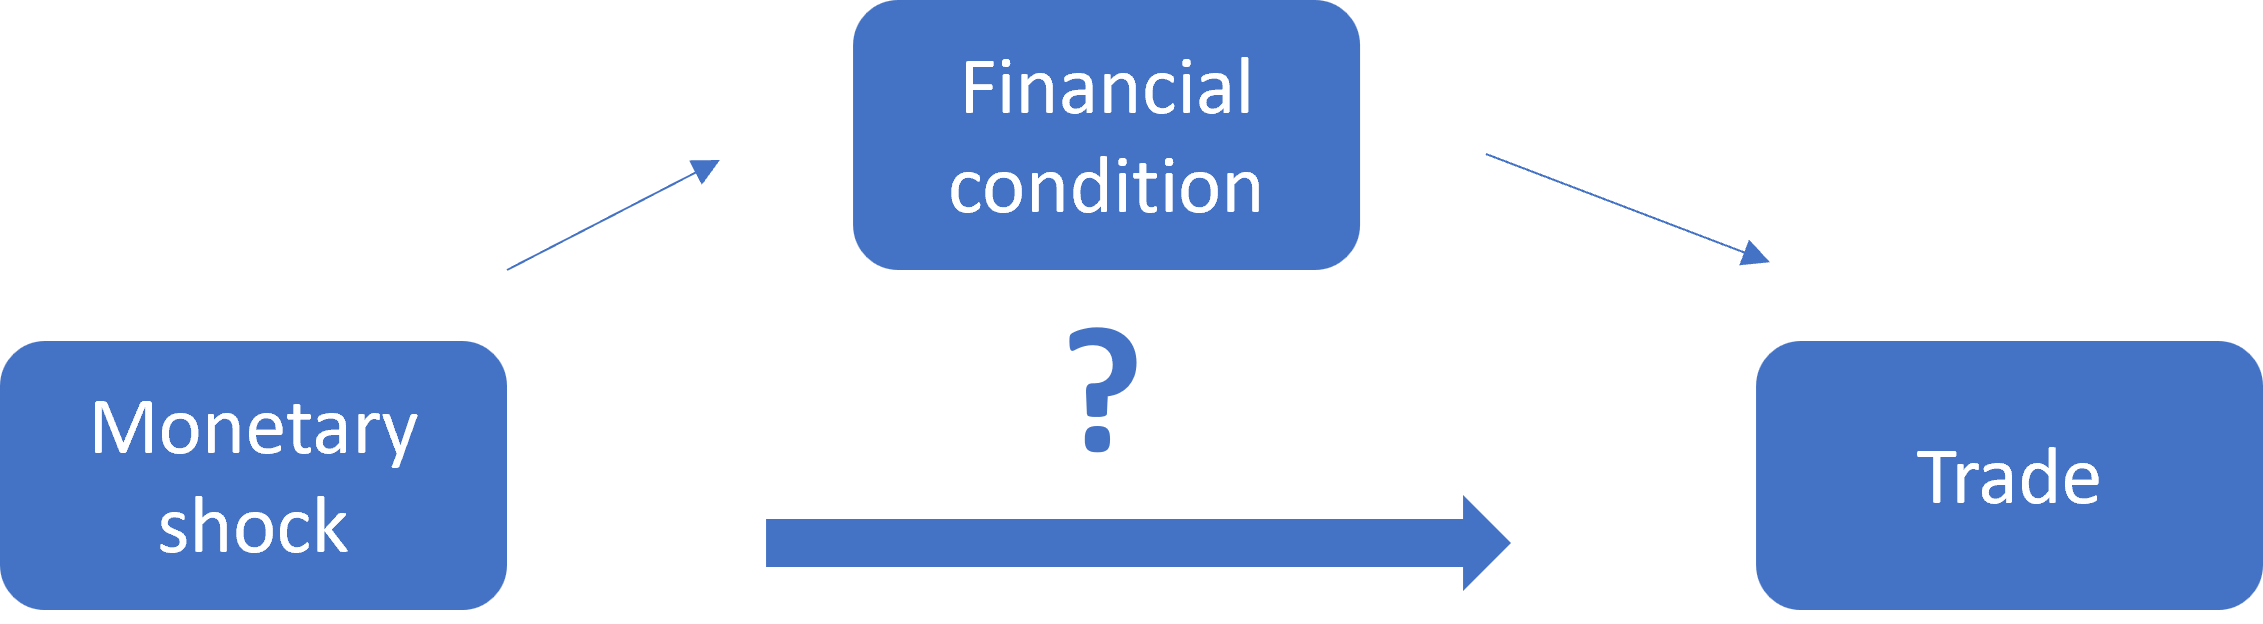
\includegraphics[width=0.7\columnwidth]{latex/drafts/pic/concepts.png}
	\label{fig.concept}
    \end{figure}
    
\begin{itemize}
    \item Financial frictions affect firms' exporting behavior (\citealp{manova2013credit}).
    \medskip
    \item Global monetary shocks (especially the US shock) are the main driver of the global financial cycle (\citealp{miranda2020us}).
    \medskip
    \item Question: how do global monetary shocks affect firms' export behavior (especially pricing) through the financial friction channel?
\end{itemize}
\end{frame}

\begin{frame}{Motivating fact}
    \begin{itemize}
        \item A tightening \textbf{US Fed} monetary policy shock will \textbf{increase} the average export price of Chinese firms.
        \begin{columns}
    	\column{0.5\columnwidth}
    	\begin{figure}[htbp]
                \centering
                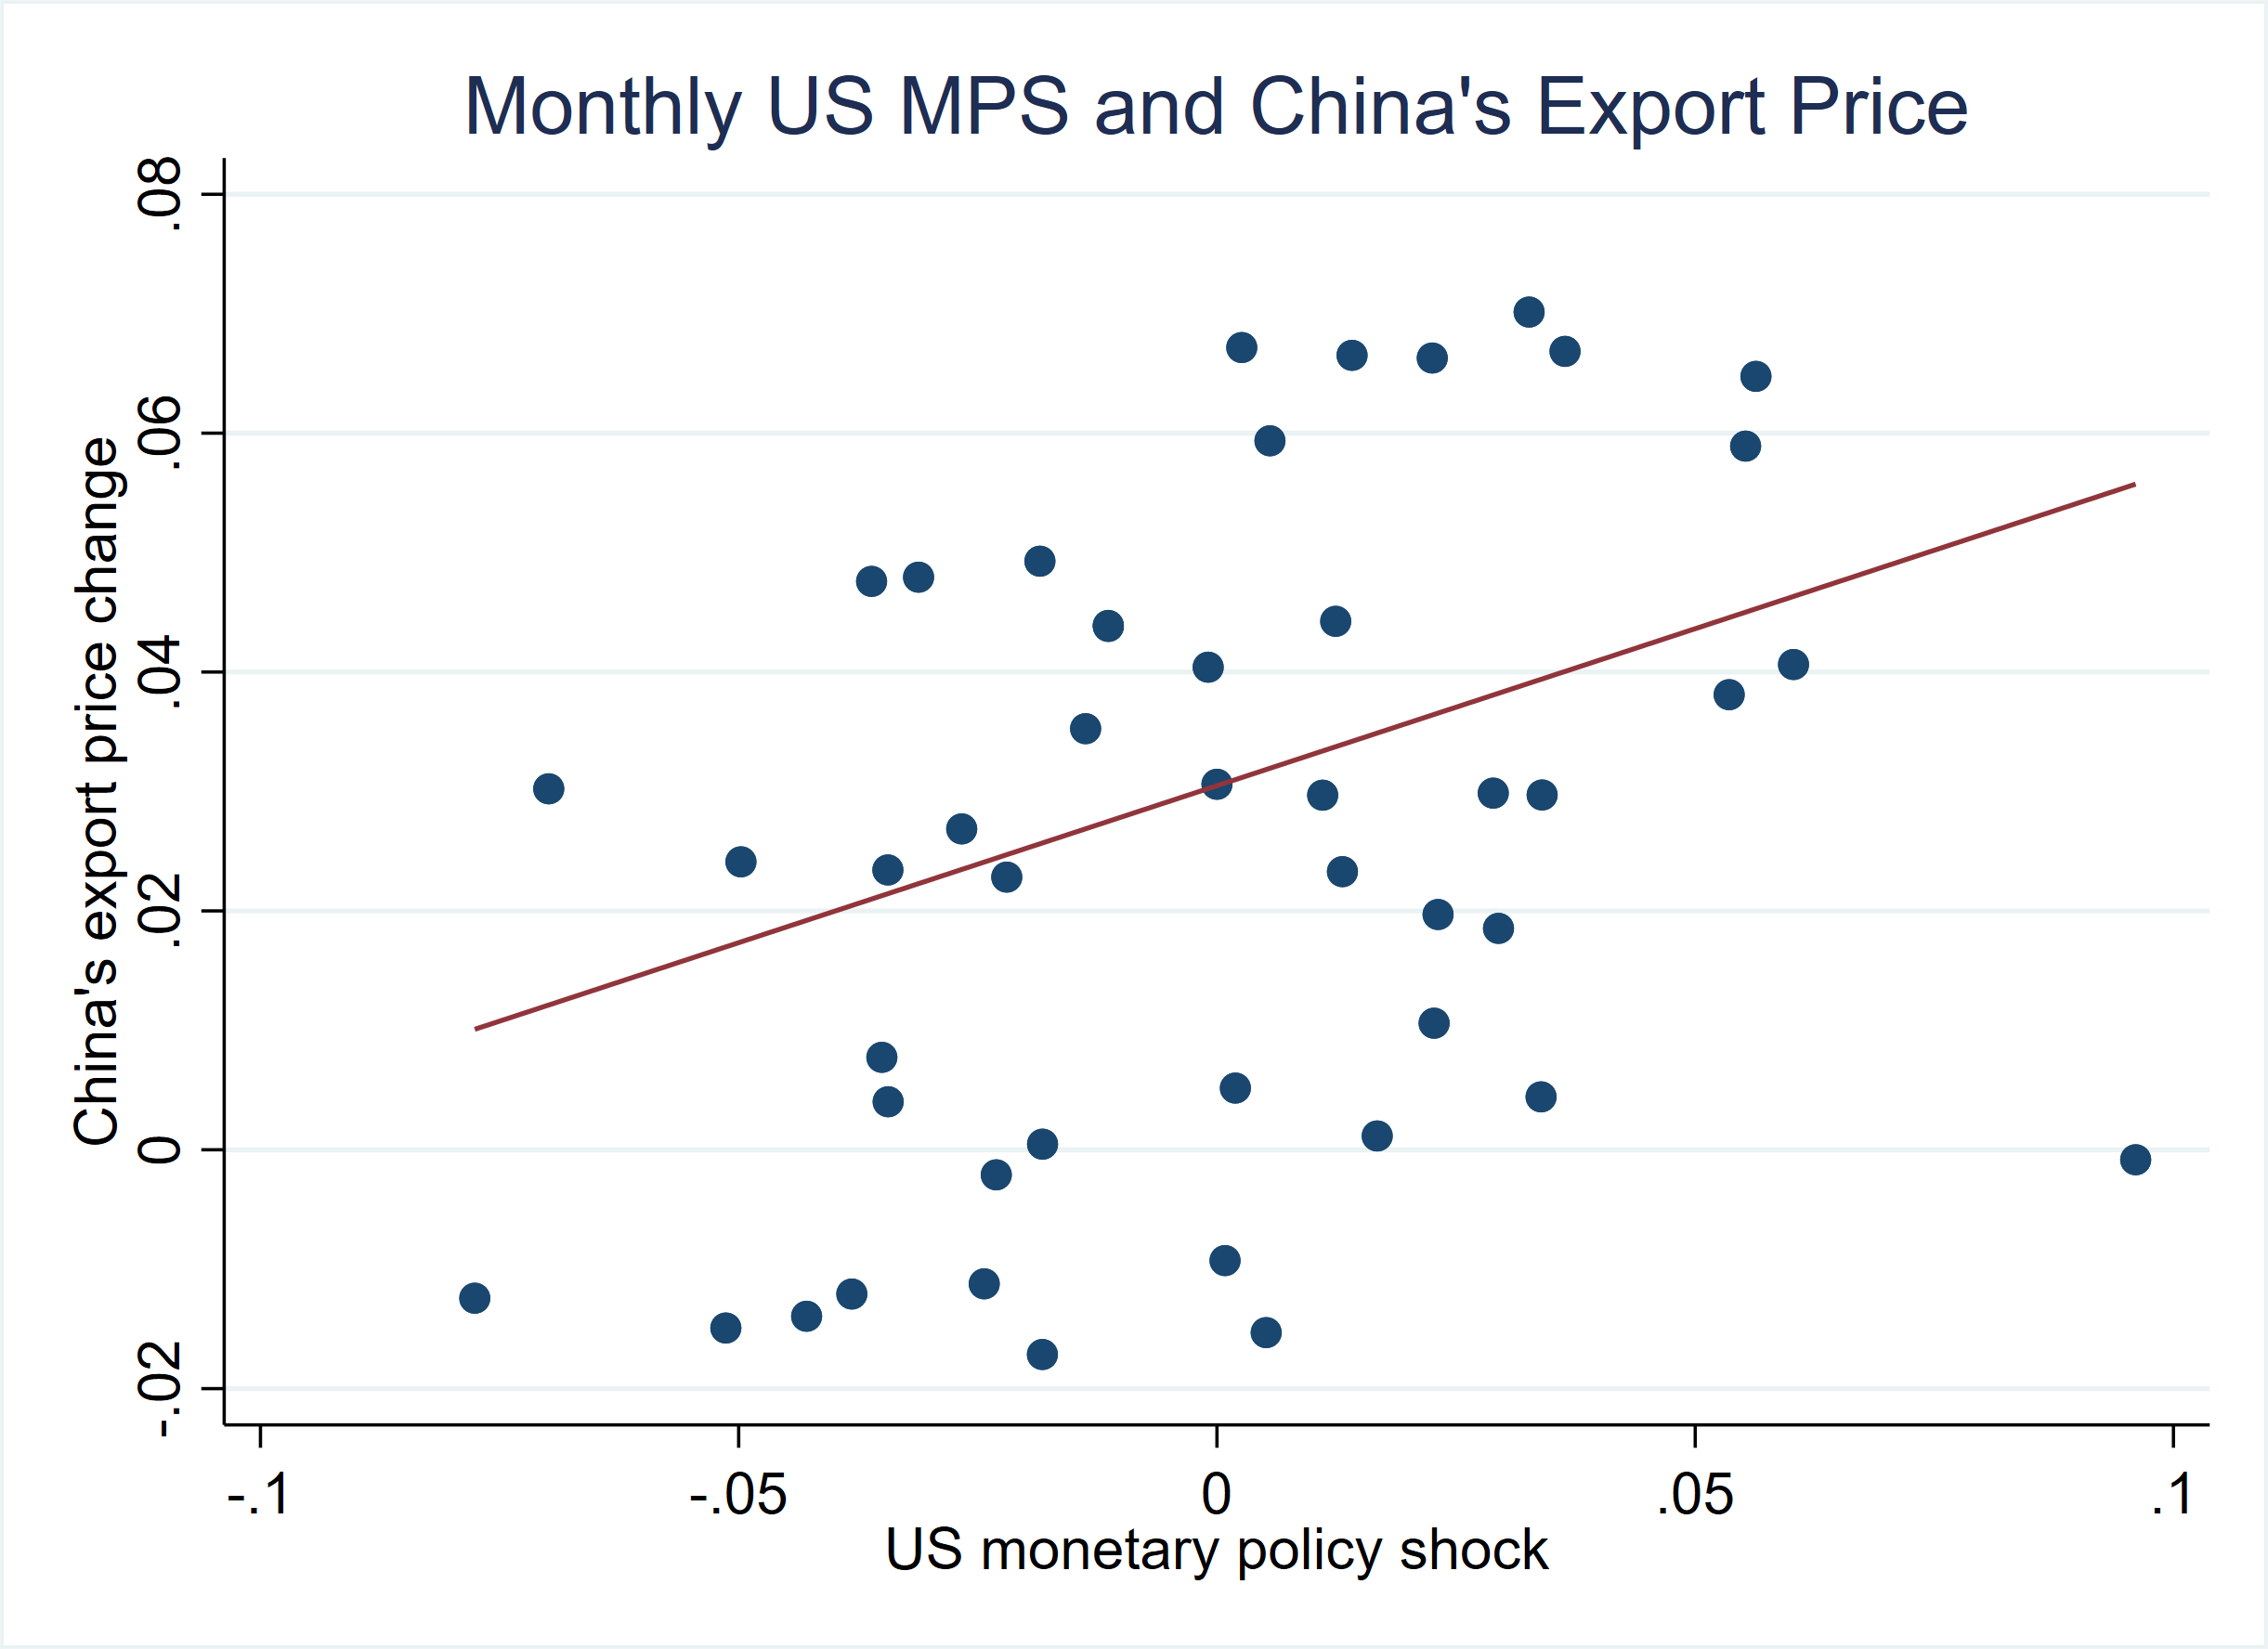
\includegraphics[width=1.1\columnwidth]{latex/slides/pic_Nov2023/brw_monthly.png}
                \label{fig.US_shock}
    	\end{figure}
    	\column{0.5\columnwidth}
    	\begin{figure}[htbp]
                \centering
                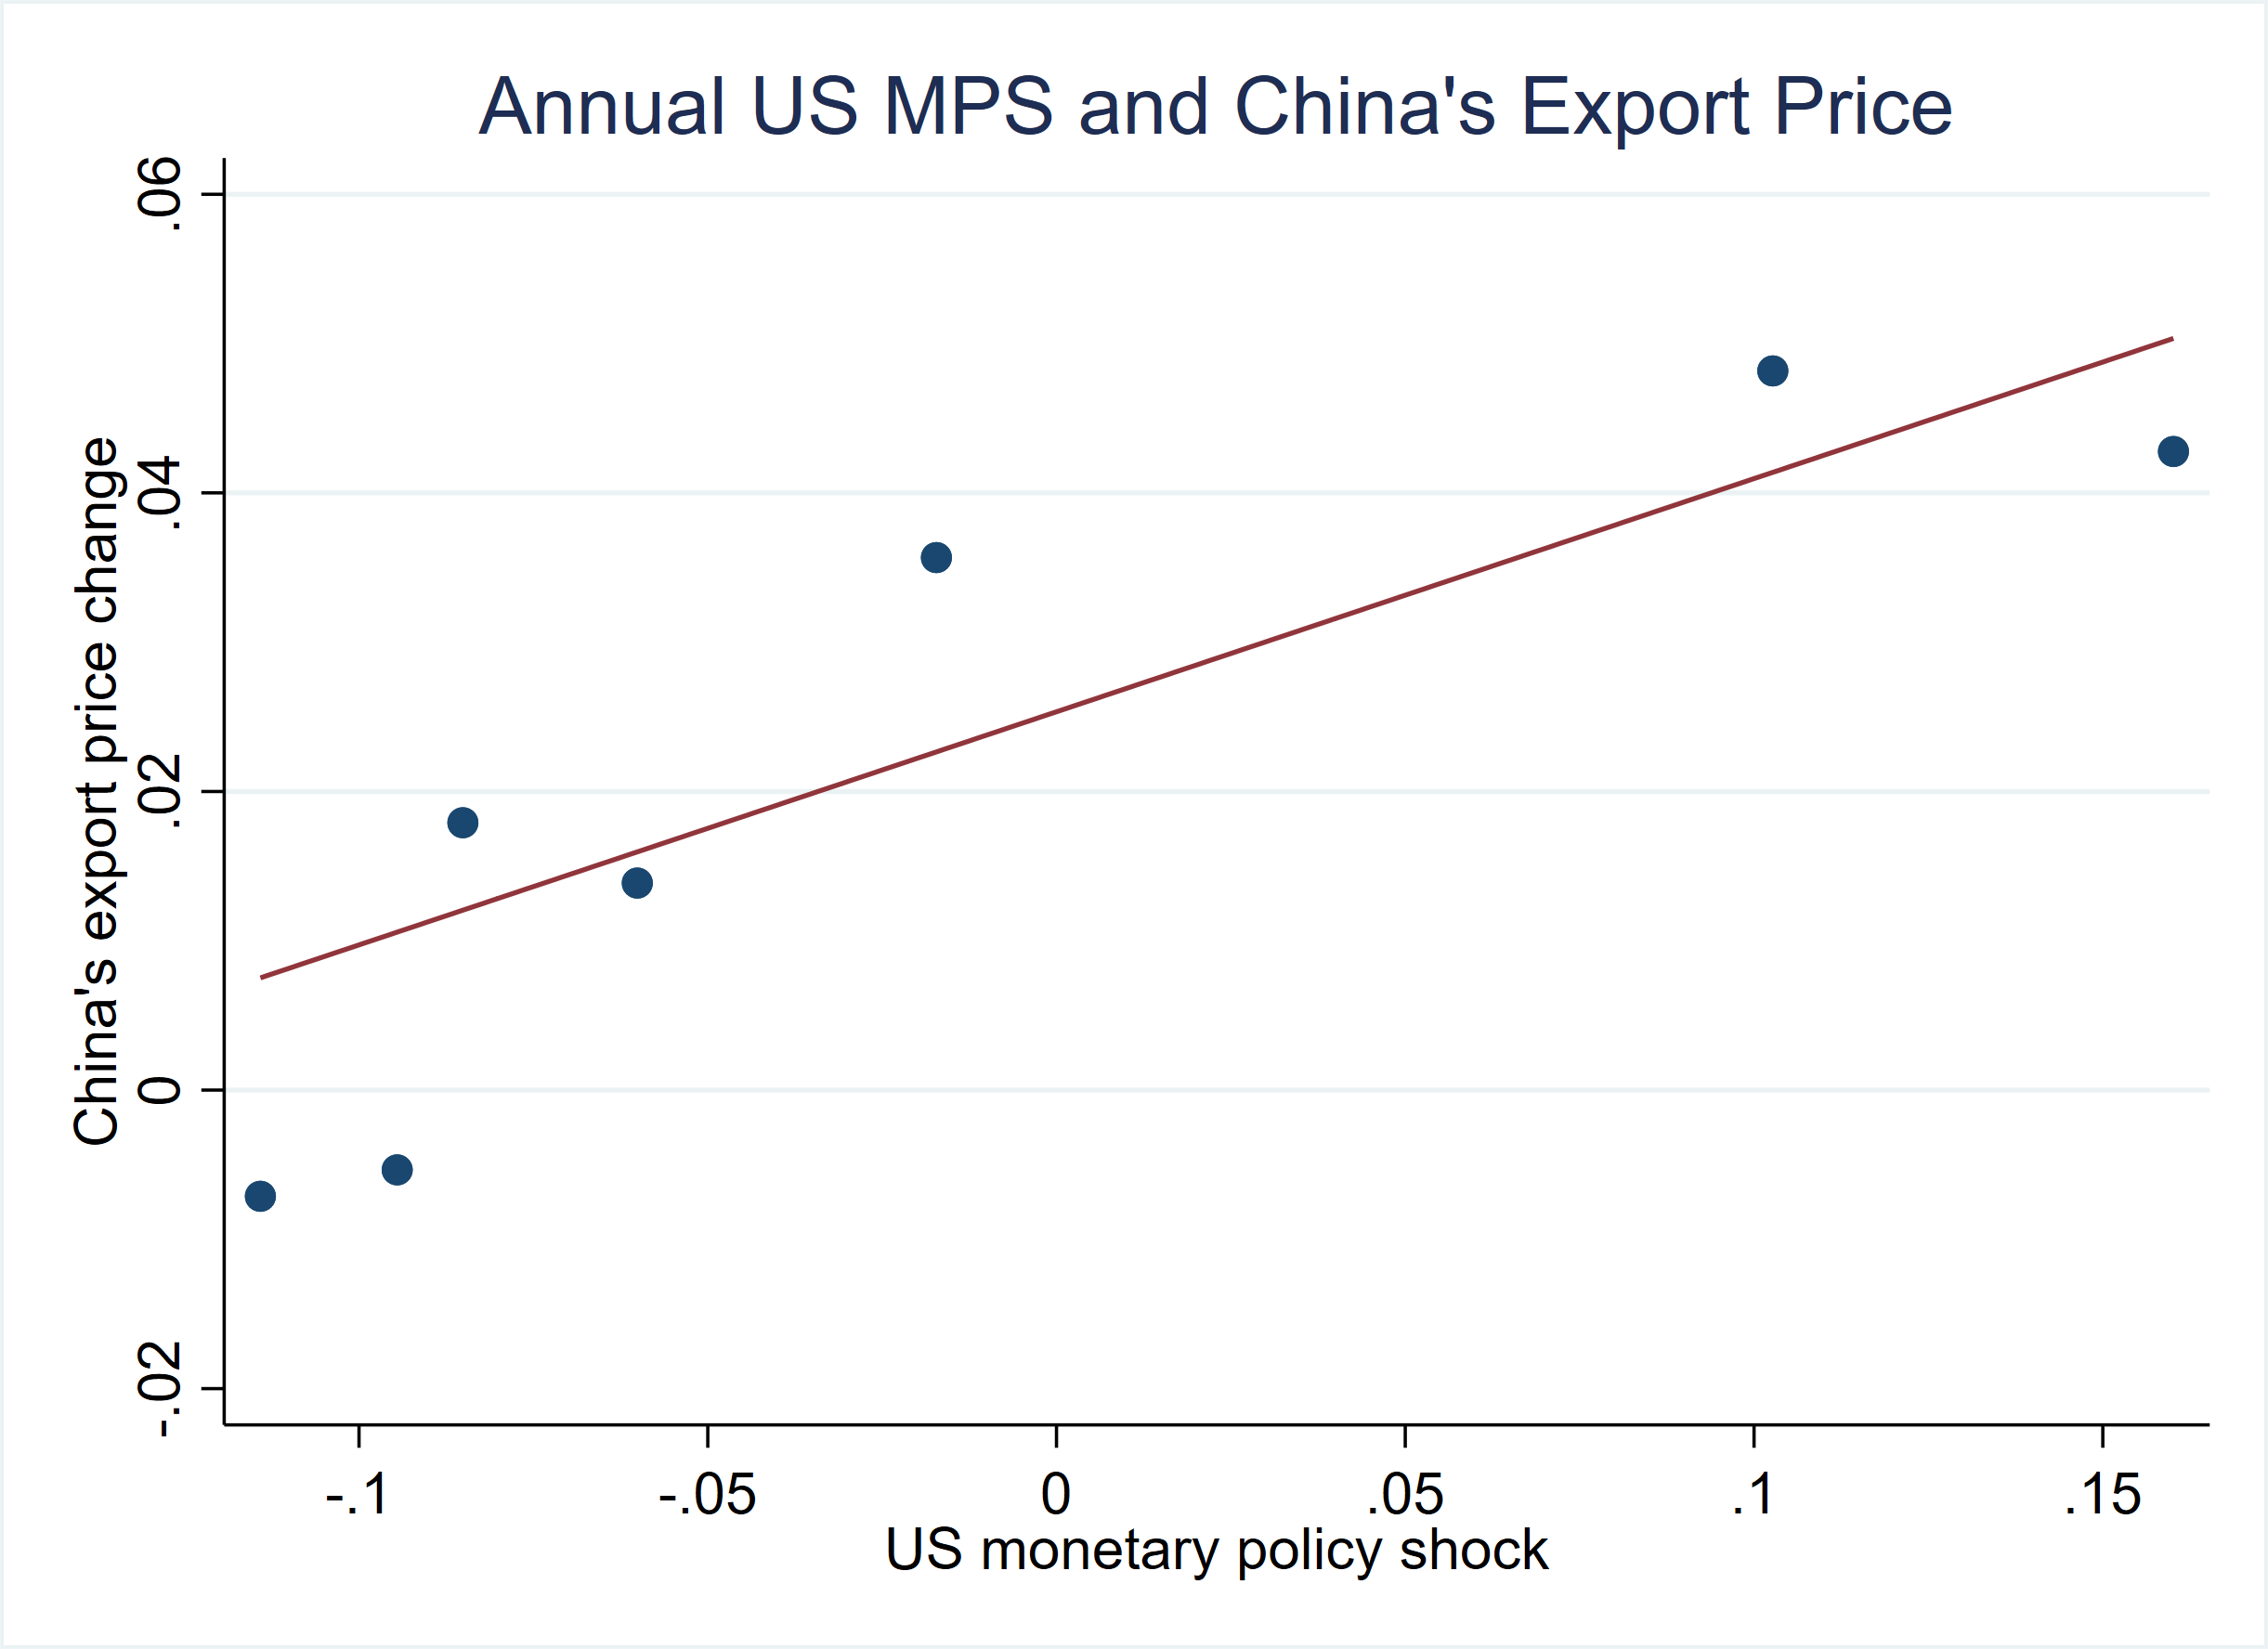
\includegraphics[width=1.1\columnwidth]{latex/slides/pic_Nov2023/brw_annual.png}
                \label{fig.EU_shock}
    	\end{figure}
        \end{columns}
    \end{itemize}
\end{frame}

\begin{frame}{This paper}

\begin{itemize}
    \item \textit{Main result}: 
        \begin{itemize}
        \item Tightening US shock increases China's export prices.
        \end{itemize}
    \medskip
    \item \textit{Channels}: 
    \begin{itemize}
        \item Shocks mainly affect marginal costs rather than markups
        \item Borrowing cost change is the main driver of marginal cost shifts
        \item Monetary tightening also deteriorates firms' liquidity conditions
        \item The impact is bigger for firms facing higher borrowing costs and tighter liquidity conditions. 
    \end{itemize}
    \medskip
    \item \textit{Model}: 
        \begin{itemize}
        \item We build a classical trade model augmented with credit constraints and external monetary shocks.
        \end{itemize}
        
\end{itemize}
\end{frame}


\begin{frame}{Literature}
\begin{itemize}
    \item Financial frictions and international trade: 
    \begin{itemize}
       \item The effect of credit constraints on firms' exports: e.g., \cite{manova2013credit}, \cite{manova2015firm}, etc.
        \item Sectoral-level export value responses: \cite{lin2018international}
        \item \textcolor{red}{This paper: how global monetary shocks affect export price through financial friction mechanism}
    \end{itemize}
    \item Determinants of export prices
        \begin{itemize}
        \item Exchange rate shocks: e.g., \cite{amiti2014importers}, \cite{auer2018quality}, etc.
        \item Firm characteristics, destinations, and trade liberalization: e.g., \cite{manova2012export}, \cite{fan2015trade}, etc.
        \item \textcolor{red}{This paper: global monetary policy shocks}
    \end{itemize}
    \item Global monetary policy spillover
        \begin{itemize}
        \item Real economy: e.g., \cite{bluedorn2011open}, \cite{di2023impact}, etc.
        \item Asset prices: e.g., \cite{rogers2014evaluating}, \cite{miranda2020us}, etc.
        \item \textcolor{red}{This paper: exporter pricing behaviors}
    \end{itemize}
\end{itemize}

\end{frame}

%%%%%%%%%%%%%%%%%%%%%%%%%%%%%%%%%%%%%%%%%%%%%%%%%%%%%%
%%%%%%%%%%%%%%%%%%%%%%%%%%%%%%%%%%%%%%%%%%%%%%%%%%%%%%
\section{II. Data and Measurements}

\begin{frame}{Data: Monetary Policy Shock}
    \begin{itemize}
        \item \cite{bu2021unified}.
        \begin{itemize}
            \item It uses \cite{fama1973risk} two-step partial-least squares estimation using FOMC announcements.
        \end{itemize}
        \item Advantages:
        \begin{enumerate}
            \item Unpredictable from past available information (exogenous);
            \item No significant information effect (pure policy shock);
            \item Bridge conventional and unconventional monetary policy regimes
        \end{enumerate}
        \item Other: \cite{nakamura2018high}, \cite{guraynak2005actions}, and \cite{jarocinski2020deconstructing}.
        \item Sample: 2000 to 2006 (84 months).
    \end{itemize}
\end{frame}

\begin{frame}{Data: Monetary Policy Shock}
    \begin{figure}[htbp]
	\centering
	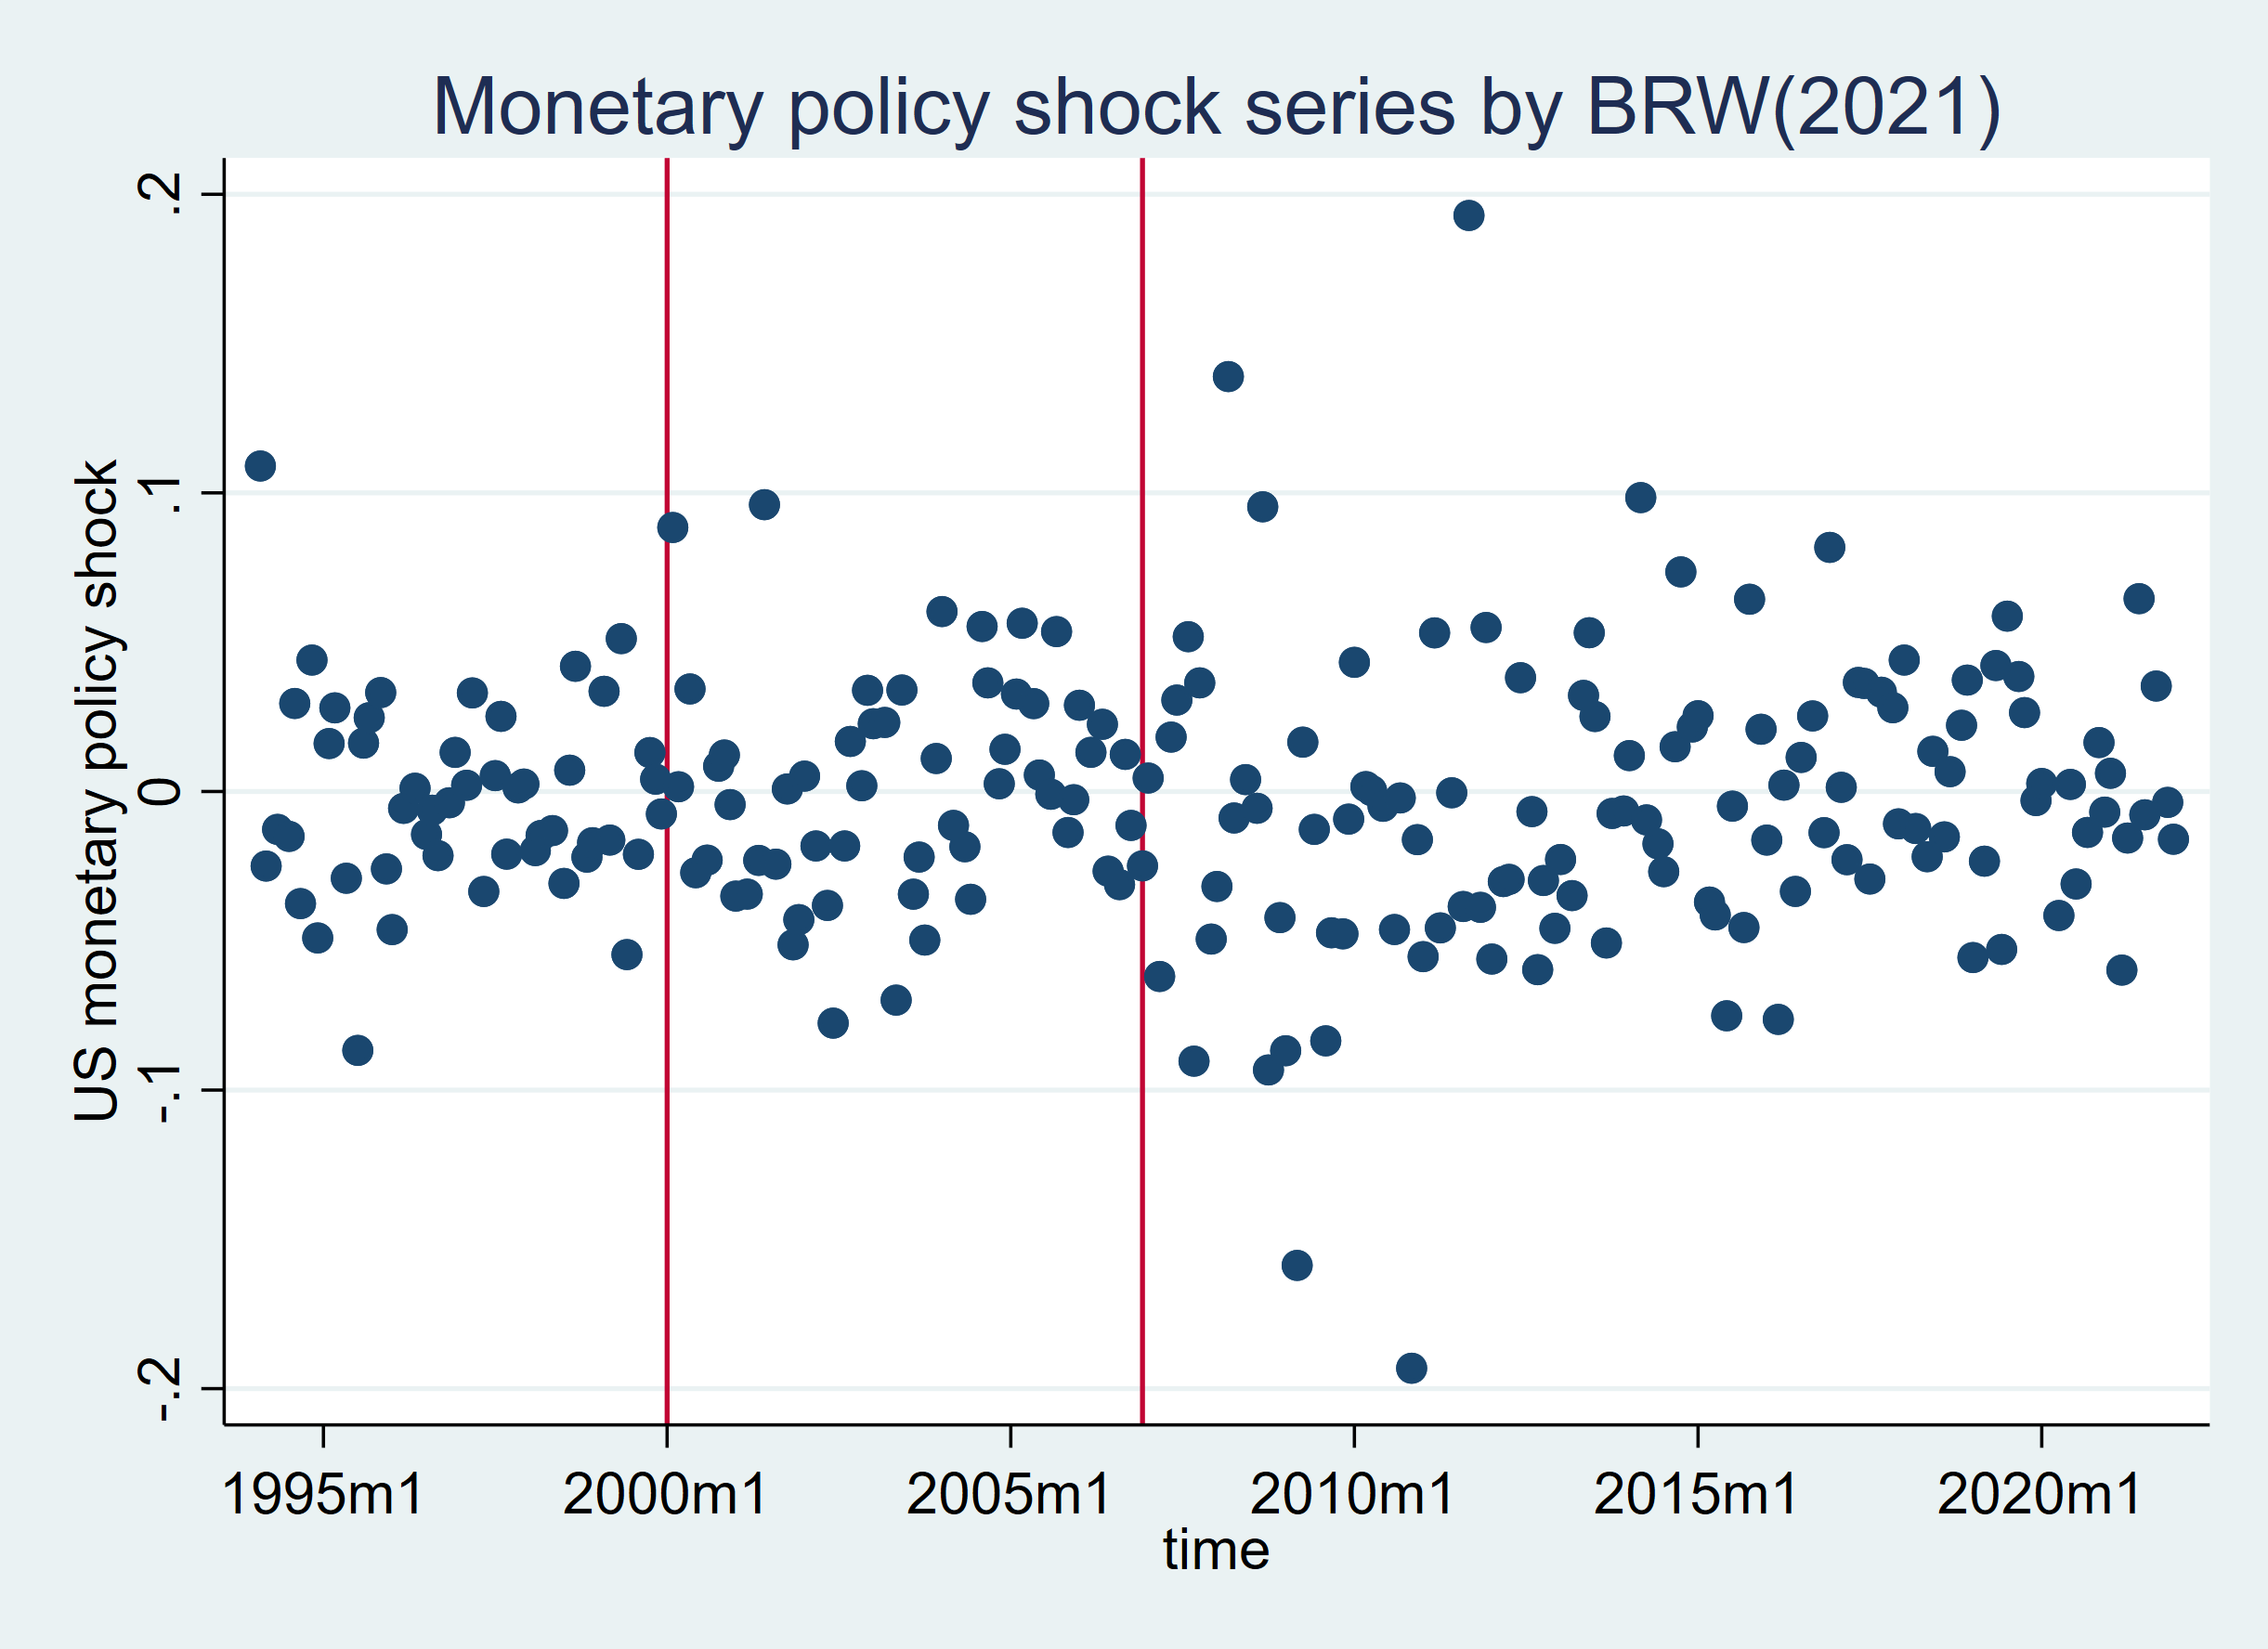
\includegraphics[width=0.9\columnwidth]{latex/drafts/pic/BRW.png}
	\label{sum.brw}
    \end{figure}
\end{frame}

\begin{frame}{Data: Firm-level and Customs data}
    \begin{itemize}
	\item Annual surveys of Chinese manufacturing firms from the National Bureau of Statistics of China
	\begin{itemize}
		\item Sample: state-owned enterprises and above-scale firms ($>$5 million RMB), 1999 to 2007 
            \item Information: balance sheet variables, especially borrowing cost and liquidity conditions
	\end{itemize}
        \medskip
        \item Monthly customs data of China
        \begin{itemize}
            \item Sample: all exporting firms (except whole-sellers), 2000-2006
            \item Information: import and export values, quantities, product names and codes, source and destination countries, and firm types
	\end{itemize}
         
    \end{itemize}
\end{frame}

\begin{frame}{Data: Summary Statistics}
    \begin{table}[htbp]
        \centering
        \caption{Summary statistics}
        \resizebox{0.9\columnwidth}{!}{
        \begin{threeparttable}
            \begin{tabular}{lccccc}
            \toprule
                    &        Mean&          SD&         p50&         p25&         p75\\
            \midrule
            $\Delta P$        &        0.03&        0.42&        0.01&       -0.11&        0.17\\
            \# HS6 Products           &        6.29&       10.31&        3.00&        2.00&        7.00\\
            Export Value (*1000 RMB)    &   129580&   372029&    19709&     3890&    80525\\
            Sales (*1000 RMB)   &   160148&  1201262&    34910&    15350&    90852\\
            Employment     &      449&     1210&      197&       96&      418\\
            $Debt$              &        0.55&        0.26&        0.56&        0.37&        0.74\\
            $IE/L$               &        0.02&        0.04&        0.01&        0.00&        0.03\\
            $Liquid$       &        0.10 &        0.29 &        0.10 &       -0.07 &        0.28\\
            $\phi^{exp}$ (Export/Sales)         &        0.46&        0.38&        0.36&        0.07&        0.89\\
            $\phi^{imp}$ (Export/Inputs)               &        0.18&        0.30&        0.01&        0.00&        0.25\\
            \midrule
            Firm-year observations        &     \multicolumn{5}{c}{270271}      \\
            \bottomrule
            \end{tabular}
            \begin{tablenotes}
        	\footnotesize
                \item Notes: This table shows the summary statistics of firms in the matched sample. The first row $\Delta P$ indicates monthly price changes, while all other rows describe annual-level firm variables. $Debt$ denotes the ratio of total liability over total assets, $IE/L$ denotes the ratio of interest expense over total liability, and $Liquid$ denotes the ratio of net liquid assets over total assets.
            \end{tablenotes}
        \end{threeparttable}
        }
        \label{tab.summary}
    \end{table}
\end{frame}

\begin{frame}{Export price index}
    \begin{itemize}
	\item We compute the unit values of each firm-product-country observation as the proxy of export prices:
        $$
        P_{ihct}=\frac{V_{ihct}\cdot NER_{US,t}}{Q_{ihct}}
        $$
        \item We construct the firm-level Tornqvist price index:
        \begin{itemize}
            \item [1] The firm-product-level price, $P_{iht}=\sum_c s_{c,iht} P_{ihct}$.
            \item [2] The firm-product-level price change: $\Delta_n \ln P_{iht} = \ln P_{iht}-\ln P_{ih(t-n)}$.
            \item [3] The firm-level price index change:
            $$
            \Delta_n \ln P_{it} = \sum _{h} \frac{s_{h,i(t-n)}+s_{h,it}}{2} \Delta_n \ln P_{iht}
            $$
            where $s_{c,iht}=V_{ihct}/V_{iht}$ and $s_{h,it}=V_{iht}/V_{it}$.
            \item In monthly regressions, the time gap $n=12$ means 12 months, 
            \item In annual regressions, the time gap $n=1$ means 1 year.
        \end{itemize}
    \end{itemize}
\end{frame}

%%%%%%%%%%%%%%%%%%%%%%%%%%%%%%%%%%%%%%%%%%%%%%%%%%%%%%
%%%%%%%%%%%%%%%%%%%%%%%%%%%%%%%%%%%%%%%%%%%%%%%%%%%%%%
\section{III. Results}

\begin{frame}{Benchmark specification}
    \begin{itemize}
        \item We study the impacts of monetary policy shocks on export prices.
        \item The baseline monthly price specification:
        \begin{equation}
            \Delta \ln P_{it} = \alpha+\beta \cdot m_{t}+ \Gamma \cdot \textbf{Z}_{it-n}+\xi_{i}+\varepsilon_{it}
         \end{equation}
        \begin{itemize}
            \item $\Delta \ln P_{it}$: the year-over-year export price index change;
            \item $m_t$: the unexpected monetary policy shock at time $t$;
            \item $\textbf{Z}_{it-n}$: a vector of firm-level lagged control terms (n=1 or 12);
            \item $\xi_{i}$: firm-level (time-invariant) fixed effects;
            \item $\beta$: coefficient of interest, the average export price response to the concurrent monetary policy surprises.
        \end{itemize}
    \end{itemize}
\end{frame}

\begin{frame}{Export price responses to monetary policy shocks}
    \begin{table}[htbp]
        \centering
        \caption{Export price responses to US monetary policy shocks}
        \resizebox{\columnwidth}{!}{
        \begin{threeparttable}
        \begin{tabular}{lcccccc}
            \toprule
            & (1)   & (2)   & (3)   & (4)   & (5)   & (6) \\
            & \multicolumn{3}{c}{Monthly $\Delta ln P_{it}$} & \multicolumn{3}{c}{Annual $\Delta ln P_{it}$}  \\
            \midrule
            $brw_t$   & 0.181*** & 0.145*** & 0.147*** & 0.136*** & 0.173*** & 0.173*** \\
                  & (0.011) & (0.010) & (0.010) & (0.007) & (0.009) & (0.009) \\
            $\Delta ln P_{it-1}$ &       & 0.301*** & 0.299*** &       & -0.297*** & -0.298***  \\
                  &       & (0.003) & (0.003) &       & (0.005) & (0.005) \\
            $Sales_{it-1}$ &       &       & -0.004*** &       &       &  0.004*\\
                  &       &       & (0.001) &       &       &  (0.003)\\
            \midrule
            Firm FE & Yes   & Yes   & Yes   & Yes   & Yes   & Yes \\
            N     & 1100399 & 940015 & 917435 & 151542 & 96296 & 96296 \\
            \bottomrule
        \end{tabular}
            \begin{tablenotes}
                \footnotesize
                \item Notes: Robust standard errors clustered at the firm level;  *, **, and *** indicate significance at 10\%, 5\%, and 1\% levels. The dependent variables in columns (1)-(3) are changes in monthly price, while columns (4)-(6) are changes in annual price. All regressions include firm fixed effects.
    	\end{tablenotes}
        \end{threeparttable}
        }
        \label{tab.baseline}
    \end{table}
\end{frame}

\begin{frame}{Robustness: Alternative shocks}
    \begin{table}[htbp]
        \centering
        \caption{Alternative monetary policy shocks}
        \resizebox{\columnwidth}{!}{
        \begin{threeparttable}
        \begin{tabular}{lcccccccc}
            \toprule
            & (1)   & (2)   & (3)   & (4)   & (5)   & (6) & (7)   & (8) \\
            & \multicolumn{2}{c}{$\Delta$ FFR} & \multicolumn{2}{c}{Nakamura \& Steinsson}  & \multicolumn{2}{c}{Acosta} & \multicolumn{2}{c}{Jarocinski \& Karadi}\\
            \midrule
            $\Delta FFR_t$ & 0.029*** & 0.025***&       &        &       &       &       &  \\
                  & (0.008) & (0.007)&       &        &       &       &       &  \\
            $NS_t$  &       &    & 0.152*** & 0.144***     &       &  \\
                  &       &   & (0.009) & (0.009)       &       &  \\
            $Target^{US}_t$ &       &       &       &       & 0.002*** & 0.002*** &       &  \\
                  &       &       &       &       & (0.000) & (0.000) &       &  \\
            $Path^{US}_t$  &       &       &       &       & 0.005*** & 0.004*** &       &  \\
                  &       &       &       &       & (0.000) & (0.000) &       &  \\
            $MP_t$ &       &       &       &       &       &       & 0.045*** & 0.068*** \\
                  &       &       &       &       &       &       & (0.006) & (0.006) \\
            $\Delta ln P_{it-1}$ &       & 0.299*** &       & 0.300*** &       & 0.299*** &       & 0.300*** \\
                  &       & (0.003) &       & (0.003) &       & (0.003) &       & (0.003) \\
            $Sales_{it-1}$ &       & -0.005*** &       & -0.004*** &       & -0.005*** &       & -0.004*** \\
                  &       & (0.001) &       & (0.001) &       & (0.001) &       & (0.001) \\
            \midrule
            Firm FE & Yes   & Yes   & Yes   & Yes   & Yes   & Yes   & Yes   & Yes \\
            N     & 1100399 & 917435 & 1100399 & 917435 & 1100399 & 917435 & 1100399 & 917435 \\
            \bottomrule
        \end{tabular}
            \begin{tablenotes}
                \footnotesize
                \item Notes: Robust standard errors clustered at the firm level;  *, **, and *** indicate significance at 10\%, 5\%, and 1\% levels. The dependent variables in all columns are changes in monthly price. Monetary policy shock measures in columns (1)-(2), (3)-(4), (5)-(6), (7)-(8) are from Fed fund rate changes, \cite{nakamura2018high}, \cite{acosta2022perceived}, and \cite{jarocinski2020deconstructing}, respectively. All regressions include firm fixed effects.
    	\end{tablenotes}
        \end{threeparttable}
        }
        \label{tab.altmps}
    \end{table}
\end{frame}

\begin{frame}[label=robustness_other]{Other robustness}
    In addition, we also adopt other robustness tests:
    \medskip
    \begin{enumerate}
        \item Alternative \textbf{aggregation levels of price index} \hyperlink{appendix_tab.altagg}{\beamergotobutton{Alternative aggregation}}
        \item Sub-sample with \textbf{only single product firms} \hyperlink{appendix_tab.single}{\beamergotobutton{Single product firms}}
        \item Alternative \textbf{standard error cluster levels and fixed effects} \hyperlink{appendix_tab.altfe}{\beamergotobutton{Alternative SE clusters and FEs}}
        \item Export prices \textbf{denominated in US dollars} \hyperlink{appendix_tab.USD}{\beamergotobutton{USD prices}}
    \end{enumerate}
\end{frame}

%%%%%%%%%%%%%%%%%%%%%%%%%%%%%%%%%%%%%%%%%%%%%%%%%%%%%%
%%%%%%%%%%%%%%%%%%%%%%%%%%%%%%%%%%%%%%%%%%%%%%%%%%%%%%

\section{IV. Mechanism}

\begin{frame}{Decomposition of prices: markup vs marginal cost}
    \begin{itemize}
        \item Components: markups and marginal costs
        \begin{itemize}
            \item Markup: the ratio of an input factor's output elasticity to its firm-specific factor payment share $\mu_{t}=\theta_{t}^{X}\left(\alpha_{t}^{X}\right)^{-1}$
            \item Literature: \cite{deloecker2012markups} and \cite{brooks2021agglomeration}.
        \end{itemize}
        \item Specification: 
        \begin{equation}
            \Delta \mu_{it} = \alpha +\beta \cdot m_{t}+ \Gamma \cdot \textbf{Z}_{it-n}+\xi_{i}+\varepsilon_{it} \label{reg.markup}
        \end{equation}
        \begin{equation}
            \Delta \ln P_{it} = \alpha+\beta \cdot m_{t}+ \gamma \cdot \Delta \mu_{it}+ \Gamma \cdot \textbf{Z}_{it-n}+\xi_{i}+\varepsilon_{i t} \label{reg.markup_int}
        \end{equation}
    \end{itemize}
\end{frame}

\begin{frame}{Price changes mainly driven by marginal costs}
    
\begin{table}[htbp]
    \centering
    \caption{Decomposition of prices: markup vs marginal cost}
    \resizebox{\columnwidth}{!}{
    \begin{threeparttable}
    \begin{tabular}{lcccccccc}
        \toprule
        & \multicolumn{4}{c}{Monthly sample} & \multicolumn{4}{c}{Annual sample}  \\
        & (1)   & (2)   & (3)   & (4)   & (5)   & (6) & (7)   & (8) \\
        \cline{2-5}  \cline{6-9}
        & $\Delta Markup_{it}$ & $\Delta ln(MC)_{it}$ & \multicolumn{2}{c}{$\Delta ln P_{it}$}  & $\Delta Markup_{it}$ & $\Delta MC_{it}$ & \multicolumn{2}{c}{$\Delta ln P_{it}$}\\
        \midrule
        $brw_t$   & -0.010 & 0.190*** & 0.149*** & 0.036*** & -0.017** & 0.174*** & 0.176*** & 0.084*** \\
              & (0.008) & (0.015) & (0.012) & (0.007) & (0.009) & (0.012) & (0.010) & (0.007) \\
        $\Delta Markup_{it}$&       &       & 0.004* &       &       &       &   0.007*    &  \\
              &       &       & (0.002) &       &       &       &   (0.004)    &  \\
        $\Delta MC_{it}$&       &       &       & 0.668*** &       &       &       &  0.472***\\
              &       &       &       & (0.004) &       &       &       &  (0.005)\\
        $\Delta ln P_{it-1}$&       &       & 0.280*** & 0.099*** &       &       &   -0.307*** & -0.163*** \\
              &       &       & (0.003) & (0.002) &       &       &   (0.005) & (0.004)  \\
        $Sales_{it-1}$ & -0.022*** & 0.019*** & -0.005*** & -0.018*** &  -0.022*** & 0.018*** & 0.006** & -0.009*** \\
              & (0.003) & (0.004) & (0.002) & (0.002) &  (0.002) & (0.003) & (0.003) & (0.002) \\
        \midrule
        Firm FE & Yes   & Yes   & Yes   & Yes   & Yes   & Yes   & Yes   & Yes \\
        N     & 830585 & 767768 & 665438 & 661680 & 110750 & 105330 & 81471 & 80831 \\
        \bottomrule
    \end{tabular}
        \begin{tablenotes}
            \footnotesize
            \item Notes: Robust standard errors clustered at the firm level;  *, **, and *** indicate significance at 10\%, 5\%, and 1\% levels. The dependent variables in columns (1), (2), (3)-(4) are changes in markup, marginal cost, and price in the monthly sample; the dependent variables in columns (5), (6), (7)-(8) are changes in markup, marginal cost, and price in the annual sample. All regressions include firm fixed effects.
	\end{tablenotes}
    \end{threeparttable}
    }
    \label{tab.markup}

\end{table}
\end{frame}

\begin{frame}{Borrowing cost and liquidity conditions}
    \begin{itemize}
        \item Hypotheses for mechanism:
        \begin{enumerate}
            \item \textbf{Borrowing cost channel}. A tightening shock increases the borrowing cost of firms
            \item \textbf{Liquidity channel}. A contractionary US monetary shock aggravates firms' liquidity conditions
        \end{enumerate}
        \item Specification:
        \begin{equation}
            \Delta F_{it} = \alpha +\beta \cdot m_{t}+ \Gamma \cdot \textbf{Z}_{it-n}+\xi_{i}+\varepsilon_{it} \label{reg.liquid}
        \end{equation}
        \item $F_{it}$ include:
        \begin{itemize}
            \item Borrowing costs: interest expense and financial cost over total liability and current liability.
            \item Liquidity conditions: working capital, net liquid asset, cash over total assets, and accounts receivable over total sales.
        \end{itemize}
    \end{itemize}
\end{frame}

\begin{frame}{Borrowing cost rises and liquidity worsens}
    \begin{table}[htbp]
        \centering
        \caption{Borrowing cost channel and liquidity channel}
        \resizebox{\columnwidth}{!}{
        \begin{threeparttable}
        \begin{tabular}{lcccccccc}
            \toprule
            &\multicolumn{4}{c}{Borrowing costs} & \multicolumn{4}{c}{Liquidity conditions} \\
            & (1)   & (2)   & (3)   & (4)   & (5)   & (6) & (7)   & (8) \\
            & $\Delta IE/L$ & $\Delta IE/CL$ & $\Delta FN/L$ & $\Delta FN/CL$ & $\Delta WC$  & $\Delta Liquid$ & $\Delta Cash$ & $\Delta Arec$ \\
            \midrule
            $brw_t$   & 0.002*** & 0.004*** & 0.002*** & 0.004*** & -0.005*** & -0.021*** & -0.007*** & -0.004** \\
                  & (0.000) & (0.001) & (0.001) & (0.001) & (0.002) & (0.002) & (0.002) & (0.002) \\
            $Sales_{it-1}$ & -0.001*** & -0.002*** & -0.003*** & -0.004*** & -0.009*** & -0.000 & -0.001*** & 0.059*** \\
                  & (0.000) & (0.000) & (0.000) & (0.000) & (0.000) & (0.001) & (0.000) & (0.001) \\
            $Debt_{it-1}$ & 0.045*** & 0.052*** & 0.080*** & 0.089*** & -0.105*** & 0.599*** & -0.005*** & -0.053*** \\
                  & (0.001) & (0.001) & (0.001) & (0.001) & (0.002) & (0.002) & (0.002) & (0.002) \\
            \midrule
            Firm FE & Yes   & Yes   & Yes   & Yes   & Yes   & Yes   & Yes   & Yes \\
            N     & 1081803 & 1056283 & 1081803 & 1056283 & 1090620 & 1090620 & 1090620 & 1090620 \\
            \bottomrule
        \end{tabular}
            \begin{tablenotes}
                \footnotesize
                \item Notes: Robust standard errors clustered at the firm level;  *, **, and *** indicate significance at 10\%, 5\%, and 1\% levels. The dependent variables in columns (1)-(4) are changes in interest expense over the total liability ratio, interest expense over the current liability ratio, total financial expense over the total liability ratio, and total financial expense over the current liability ratio, respectively. The dependent variables in columns (5)-(8) are changes in working capital over total asset ratio, net liquidity asset over total asset ratio, cash over total asset ratio, and accounts receivable over sales ratio, respectively. All regressions include firm fixed effects.
    	\end{tablenotes}
        \end{threeparttable}
        }
        \label{tab.liquid}
    \end{table}
\end{frame}

\begin{frame}{Bigger impacts with higher costs and tighter liquidity}
    \begin{table}[htbp]
        \centering
        \caption{Interactions with borrowing cost and liquidity}
        \resizebox{0.78\columnwidth}{!}{
        \begin{threeparttable}
        \begin{tabular}{lcccccccc}
            \toprule
            & (1)   & (2)   & (3)   & (4)   & (5)   & (6)   & (7)   & (8) \\
        \midrule
        $brw_t$ & 0.107*** & 0.109*** & 0.087*** & 0.092*** & 0.351*** & 0.236*** & 0.510*** & 0.129*** \\
              & (0.017) & (0.017) & (0.033) & (0.031) & (0.097) & (0.022) & (0.082) & (0.025) \\
        $brw_t \times IE/L_{st}$ & 6.580*** &       &       &       &       &       &       &  \\
              & (1.977) &       &       &       &       &       &       &  \\
        $brw_t \times IE/CL_{st}$ &       & 5.415*** &       &       &       &       &       &  \\
              &       & (1.701) &       &       &       &       &       &  \\
        $brw_t \times FN/L_{st}$ &       &       & 4.203** &       &       &       &       &  \\
              &       &       & (2.112) &       &       &       &       &  \\
        $brw_t \times FN/CL_{st}$ &       &       &       & 3.466** &       &       &       &  \\
              &       &       &       & (1.768) &       &       &       &  \\
        $brw_t \times WC_{st}$ &       &       &       &       & -0.331** &       &       &  \\
              &       &       &       &       & (0.159) &       &       &  \\
        $brw_t \times Liquid_{st}$ &       &       &       &       &       & -1.137*** &       &  \\
              &       &       &       &       &       & (0.270) &       &  \\
        $brw_t \times Cash_{st}$ &       &       &       &       &       &       & -2.226*** &  \\
              &       &       &       &       &       &       & (0.498) &  \\
        $brw_t \times Arec_{st}$ &       &       &       &       &       &       &       & 0.167 \\
              &       &       &       &       &       &       &       & (0.218) \\
        $\Delta ln P_{it-1}$ & 0.299*** & 0.299*** & 0.299*** & 0.299*** & 0.299*** & 0.299*** & 0.299*** & 0.299*** \\
              & (0.003) & (0.003) & (0.003) & (0.003) & (0.003) & (0.003) & (0.003) & (0.003) \\
        $Sales_{it-1}$ & -0.004*** & -0.004*** & -0.004*** & -0.004*** & -0.004*** & -0.004*** & -0.004*** & -0.004*** \\
              & (0.001) & (0.001) & (0.001) & (0.001) & (0.001) & (0.001) & (0.001) & (0.001) \\
        \midrule
        Firm FE & Yes   & Yes   & Yes   & Yes   & Yes   & Yes   & Yes   & Yes \\
        N     & 917435 & 917435 & 917435 & 917435 & 917435 & 917435 & 917435 & 917435 \\
            \bottomrule
        \end{tabular}
            \begin{tablenotes}
                \footnotesize
                \item Notes: Robust standard errors clustered at the firm level;  *, **, and *** indicate significance at 10\%, 5\%, and 1\% levels. The interaction terms in columns (1)-(8) are the industry-level average interest expense over the total liability ratio, interest expense over the current liability ratio, total financial expense over the total liability ratio, total financial expense over the current liability ratio, working capital over total asset ratio, net liquidity asset over total asset ratio, cash over total asset ratio, and accounts receivable over sales ratio. All regressions include firm fixed effects.
    	\end{tablenotes}
        \end{threeparttable}
        }
        \label{tab.non-linearity}
    \end{table}
\end{frame}

\begin{frame}{Other production costs responses are insignificant}
    \begin{table}[htbp]
        \centering
        \caption{Discussion about other production costs}
        \resizebox{0.9\columnwidth}{!}{
        \begin{threeparttable}
        \begin{tabular}{lccccc}
            \toprule
            & (1)   & (2)   & (3)   & (4)   & (5) \\
            & $\Delta Input/Sales$ & $\Delta Wage/Sales$ & \multicolumn{3}{c}{$\Delta ln P_{it}$}\\
            \midrule
            $brw_t$   & 0.403 & -0.164 & 0.142*** & 0.159*** & 0.154*** \\
                  & (0.263) & (0.135) & (0.011) & (0.013) & (0.014) \\
            $brw_t \times Input/Sales $ &       &       & 0.007 &       &       \\
                  &       &       & (0.005) &       &      \\
            $brw_t \times Wage/Sales $ &       &       &       & -0.108 &         \\
                  &       &       &       & (0.078) &     \\
            $brw_t \times \phi^{imp}_t$ &       &       &       &       & -0.027  \\
                  &       &       &       &       & (0.032)  \\
            $Debt_{it_1}$ & 0.436** & 0.241 &       &       &       \\
                  & (0.180) & (0.162) &       &       &    \\
            $\Delta ln P_{it-1}$ &       &       & 0.299*** & 0.299*** & 0.299***  \\
                  &       &       & (0.003) & (0.003) & (0.003)  \\
            $Sales_{it-1}$ &  1.075*** & -0.044   & -0.004*** & -0.004*** & -0.004*** \\
                  &  (0.262) & (0.187) & (0.001) & (0.001) & (0.001) \\
            \midrule
            Firm FE & Yes   & Yes   & Yes   & Yes   & Yes \\
            N     & 1090620 & 1090620 & 917435 & 917435 & 917435 \\
            \bottomrule
        \end{tabular}
            \begin{tablenotes}
                \footnotesize
                \item Notes: Robust standard errors clustered at the firm level;  *, **, and *** indicate significance at 10\%, 5\%, and 1\% levels. The dependent variables in columns (1)-(2) are changes in intermediate input cost over sales ratio and wage expense over sales ratio, respectively. The dependent variables in columns (3)-(7) are changes in monthly price. All regressions include firm fixed effects.
    	\end{tablenotes}
        \end{threeparttable}
        }
        \label{tab.other}
    \end{table}
\end{frame}

\begin{frame}{Verification: processing trade responses are weaker}
    \begin{itemize}
        \item \textbf{Processing trade}: imports raw materials and intermediate inputs from a foreign firm for processing and re-exports to the same firm. It is less dependent on external financing (\cite{manova2016firms}).
    \end{itemize}
    \begin{table}[h]
        \centering
        \caption{Ordinary trade vs processing trade}
        \resizebox{0.85\columnwidth}{!}{
        \begin{threeparttable}
        \begin{tabular}{lcccccc}
            \toprule
            & (1)   & (2)   & (3)   & (4)   & (5)   & (6) \\
              & \multicolumn{2}{c}{Ordinary trade}  & \multicolumn{2}{c}{Processing trade} & \multicolumn{2}{c}{Comparison}\\
            \midrule
            $brw_t$   & 0.201*** & 0.186*** & 0.098*** & 0.065*** & 0.225*** & 0.185*** \\
                  & (0.018) & (0.019) & (0.019) & (0.016) & (0.016) & (0.016) \\
            $brw_t \times process_{it}$ &       &       &       &       & -0.102*** & -0.085*** \\
                  &       &       &       &       & (0.024) & (0.023) \\
            $\Delta ln P_{it-1}$ &       & 0.190*** &       & 0.473*** &       & 0.299*** \\
                  &       & (0.003) &       & (0.005) &       & (0.003) \\
            $Sales_{it-1}$ &       & -0.004* &       & -0.009*** &       & -0.004*** \\
                  &       & (0.002) &       & (0.002) &       & (0.001) \\
            Firm FE & Yes   & Yes   & Yes   & Yes   & Yes   & Yes \\
            N     & 499418 & 391336 & 283952 & 242587 & 1100399 & 917435 \\
            \bottomrule
        \end{tabular}
            \begin{tablenotes}
                \footnotesize
                \item Notes: Robust standard errors clustered at the firm level;  *, **, and *** indicate significance at 10\%, 5\%, and 1\% levels. The dependent variables in columns (1)-(3) are changes in monthly price denominated in the US dollar, while columns (4)-(6) are changes in annual price denominated in the US dollar. All regressions include firm fixed effects.
    	\end{tablenotes}
        \end{threeparttable}
        }
        \label{tab.process}
    \end{table}
\end{frame}

\begin{frame}{Alternative explanations}
    \begin{itemize}
        \item \textbf{Demand shift}: Will global demand shift to Chinese goods in the global recession because of their lower quality?
        \begin{itemize}
            \item \textbf{Homogeneous}: reference priced or traded on an organized exchange.
        \end{itemize}
    \end{itemize}
    \begin{table}[htbp]
        \centering
        \caption{Price response for homogeneous goods}
        \resizebox{0.9\columnwidth}{!}{
        \begin{threeparttable}
        \begin{tabular}{lcccccccc}
            \toprule
            & (1)   & (2)   & (3)   & (4)   & (5)   & (6)   & (7)   & (8) \\
            & \multicolumn{4}{c}{Conservative classification} & \multicolumn{4}{c}{Liberal classification} \\
            \midrule
            $brw_t$   & 0.170*** & 0.126*** & 0.149*** & 0.114*** & 0.168*** & 0.124*** & 0.148*** & 0.115*** \\
              & (0.011) & (0.011) & (0.012) & (0.012) & (0.012) & (0.011) & (0.013) & (0.012) \\
            $brw_t \times ToE_{it} $ & 0.152 & 0.112 &       &    & 0.263*** & 0.242***    &       &  \\
              & (0.128) & (0.125) &       &      & (0.086) & (0.082)     &       &  \\
            $brw_t \times Ref_{it} $ &       &       & 0.208*** & 0.125*** &       &    & 0.167*** & 0.082*** \\
              &       &       & (0.033) & (0.032) &       &         & (0.031) & (0.030)\\
            $\Delta ln P_{it-1}$ &       & 0.298*** &       & 0.298*** &       & 0.298*** &       & 0.298*** \\
              &       & (0.003) &       & (0.003) &       & (0.003) &       & (0.003) \\
            $Sales_{it-1}$ &       & 0.004*** &       & 0.004*** &       & 0.004*** &       & 0.004*** \\
              &       & (0.001) &       & (0.001) &       & (0.001) &       & (0.001) \\
        \midrule
        Firm FE & Yes   & Yes   & Yes   & Yes   & Yes   & Yes   & Yes   & Yes \\
        N     & 1014106 & 850174 & 1014106 & 850174 & 1014106 & 850174 & 1014106 & 850174 \\
            \bottomrule
        \end{tabular}
            \begin{tablenotes}
                \footnotesize
                \item Notes: Robust standard errors clustered at the firm level;  *, **, and *** indicate significance at 10\%, 5\%, and 1\% levels. The variables "ToE" and "Ref" represent the value share of goods traded on an organized exchange and the value share of reference-priced goods of firm $i$. Columns (1)-(4) use the "conservative" classification, while columns (5)-(8) use the "liberal" classification, both referring to \cite{rauch1999networks}. All regressions include firm fixed effects.
    	\end{tablenotes}
        \end{threeparttable}
        }
        \label{tab.rauch}
    \end{table}
\end{frame}

\begin{frame}[label=alt_erpt]{Alternative explanations}
    \begin{itemize}
        \item \textbf{Exchange rate pass-through}: Is the export price increase driven by RMB depreciation?
        \item Refutation:
        \begin{enumerate}
            \item Control the change of bilateral real exchange rate. \hyperlink{appendix_tab.altagg}{\beamergotobutton{Alternative aggregation}}
            \item Complete export exchange rate pass-through (about 95\%), as in \cite{li2015exchange}.
            \item Most samples are in the fixed regime. US tightening shock will cause the RMB to appreciate vs third-country currencies.
        \end{enumerate}
        
    \end{itemize}
\end{frame}

%%%%%%%%%%%%%%%%%%%%%%%%%%%%%%%%%%%%%%%%%%%%%%%%%%%%%%
%%%%%%%%%%%%%%%%%%%%%%%%%%%%%%%%%%%%%%%%%%%%%%%%%%%%%%

\section{V. More Discussion}

\begin{frame}{EU shocks produce weaker effects}
\begin{itemize}
    \item Special role of US policy as a main driver of the global financial cycle.
\end{itemize}
    
    \begin{table}[htbp]
        \centering
        \caption{Export price responses to EU monetary policy shocks}
        \resizebox{0.9\columnwidth}{!}{
        \begin{threeparttable}
        \begin{tabular}{lcccccc}
            \toprule
            & (1)   & (2)   & (3)   & (4)   & (5)   & (6) \\
            & \multicolumn{3}{c}{Miranda-Agrippino \& Nenova} & \multicolumn{3}{c}{Jarocinski \& Karadi}  \\
            \midrule
            $m^{EU}_t$ & -0.002*** & -0.001*** & -0.001*** & -0.050*** & 0.002 & -0.002 \\
                  & (0.000) & (0.000) & (0.000) & (0.011) & (0.011) & (0.011)\\  
            $\Delta ln P_{it-1}$ &       & 0.301*** & 0.300*** &       & 0.301*** & 0.300*** \\
                  &       & (0.003) & (0.003) &       & (0.005) & (0.005) \\
            $Sales_{it-1}$ &       &       & -0.004*** &       &       & -0.004*** \\
                  &       &       & (0.001) &       &       & (0.001) \\
            \midrule
            Firm FE & Yes   & Yes   & Yes   & Yes   & Yes   & Yes \\
             N     & 1100399 & 940015 & 917435 & 1100399 & 940015 & 917435 \\
            \bottomrule
        \end{tabular}
        \begin{tablenotes}
            \footnotesize
            \item Notes: Robust standard errors clustered at the firm level;  *, **, and *** indicate significance at 10\%, 5\%, and 1\% levels. Monetary policy shocks here are from the European Central Bank. The shock in columns (1)-(3) are obtained from \cite{miranda2022tale}, while columns (4)-(6) are  from \cite{jarocinski2020deconstructing}. All regressions include firm fixed effects.
    	\end{tablenotes}
        \end{threeparttable}
        }
        \label{tab.EU}
    \end{table}

\end{frame}

\begin{frame}{Floating exchange rate regime is a buffer}

    \begin{table}[htbp]
        \centering
        \caption{Exchange rate regime shift: before and after July 2005}
        \resizebox{0.9\columnwidth}{!}{
        \begin{threeparttable}
        \begin{tabular}{lcccccc}
            \toprule
            & (1)   & (2)   & (3)   & (4)   & (5)   & (6) \\
            & \multicolumn{3}{c}{Fixed regime: before July 2005} & \multicolumn{3}{c}{Floating regime: after July 2005}  \\
            \midrule
            $brw_t$   & 0.189*** & 0.138*** & 0.138*** & 0.031 & 0.108*** & 0.080*** \\
                  & (0.012) & (0.012) & (0.012) & (0.022) & (0.023) & (0.023) \\
            $\Delta ln P_{it-1}$ &       & 0.288*** & 0.287*** &       & 0.186*** & 0.182*** \\
                  &       & (0.003) & (0.003) &       & (0.004) & (0.004) \\
            $Sales_{it-1}$ &       &       & 0.000 &       &       & -0.025*** \\
                  &       &       & (0.002) &       &       & (0.004) \\
            \midrule
            Firm FE & Yes   & Yes   & Yes   & Yes   & Yes   & Yes \\
            N     & 708254 & 609726 & 594891 & 389776 & 328076 & 320432 \\
            \bottomrule
        \end{tabular}
            \begin{tablenotes}
                \footnotesize
                \item Notes: Robust standard errors clustered at the firm level;  *, **, and *** indicate significance at 10\%, 5\%, and 1\% levels. Columns (1)-(3) cover the period from January 2000 to July 2005, while columns (4)-(6) cover the period from August 2005 to December 2006. All regressions include firm fixed effects.
    	\end{tablenotes}
        \end{threeparttable}
        }
        \label{tab.regime}
    \end{table}
\end{frame}

%%%%%%%%%%%%%%%%%%%%%%%%%%%%%%%%%%%%%%%%%%%%%%%%%%%%%%
%%%%%%%%%%%%%%%%%%%%%%%%%%%%%%%%%%%%%%%%%%%%%%%%%%%%%%
\section{VI. Model}

\begin{frame}{Preference}

Follow Meliz (2003) and Manova (2012). The source and destination countries are denoted by $i$ and $j$, respectively. Consumers in the country $j$ can access a set of goods $X_j$. \\
\medskip
A representative consumer in country $j$ has a constant elasticity of substitution (CES) utility:

\begin{equation}
U_j=(\int_{\omega \in \Omega_j} [\chi_{ij}(\omega)]^{\frac{\sigma-1}{\sigma}} d\omega\ )^\frac{\sigma}{\sigma-1}
\end{equation}

where $\chi_{ij}$ is country $j$’s quantity consumed of variety $\omega$ originated from country $i$, and $\sigma$ $>$ 1 is the elasticity of substitution between varieties. 

\end{frame}



\begin{frame}{Demand}

Consumer optimization yields the following demand function for variety $\omega$:

\begin{equation}
\chi_{ij}(\omega)=\frac{p_{ij}(\omega)^{-\sigma}}{P_j^{-\sigma}} Y_j
\end{equation}


where $p_{ij}(\omega)$ is the price of variety $\omega$, $P_j=(\int_{\omega \in \Omega_j} [p_{ij}(\omega)]^{1-\sigma} d \omega)^{\frac{1}{1-\sigma}}$ is an aggregate price index in country $j$, and $Y_j$ represents the total expenditure of country $j$.
\vfill
Assumption: $Y_j=\bar{Y_j}+\rho_{Y}^j m+\epsilon_Y$, where $\bar{Y_j}$ is a trend component of $Y_j$, $\rho_{Y}^j<0$, $\epsilon_Y$ is a random error, and a positive $m$ means a tightening shock.

\end{frame}



\begin{frame}{Exporting firm}

\textbf{Assumption}: working capital constraint
\vfill

A fraction $\delta_i$ ($\in$ [0, 1]) of the input costs should be borrowed from outside financial institutions and paid in advance.

$$
\delta_i \equiv 1-c_i^\gamma-\zeta_i
$$

where $c_i$ $\in$ [0, 1] is the liquidity condition, $\gamma>0$ reflects the elasticity, and $\zeta_i$ $\in$ [0, 1] is trade credit. We assume:

$$
c_i=\bar{c_i}+\rho_c^i m+\epsilon_c^i,\ \rho_c^i<0
$$
$$
\zeta_i=\bar{\zeta_i}+\rho_\zeta^i m+\epsilon_t^i,\ \rho_\zeta^i<0
$$.

\end{frame}


\begin{frame}{Exporting firm}

\textbf{The production function}:

$$
y_i= \phi_i L_i
$$

where $\phi_i$ is productivity and $L_i$ is input.The firm in country $i$ minimizes its cost to satisfy the demand in the country $j$, $\chi_{ij}(\omega)=\frac{p_{ij}(\omega)^{-\sigma}}{P_j^{-\sigma}} Y_j$.
\vfill

\textbf{The cost function}:

$$
C_{ij}=\frac{w_i(1-\delta_i+\delta_i R_i)}{\phi_i} \frac{p_{ij}(\omega)^{-\sigma}}{P_j^{-\sigma}} Y_j
$$ 

$w_i$ is the price of input and $R_i$ is the gross borrowing interest rate in country $i$. We assume $R_i=\bar{R_i}+\rho_R^i m+\epsilon_R^i$, $\rho_R^i>0$. To capture the demand side effect, we allow the input price to fluctuate in response to global monetary shocks: $w_i=\bar{w_i}+\rho_w^i m + \epsilon_w^i$, $\rho_w^i<0$.

\end{frame}


\begin{frame}{Firm's problem}

\textbf{Assumption}: firms cannot borrow more than a fraction $\theta$ of the expected cash flow from exporting, and it is smaller when $R$ is higher (higher interest rates imply higher risk).$\theta=R^{-\nu}$, where $\nu>0$.
\vfill 

$$
\max_{p} \ (p- \frac{\tau w(1-\delta+\delta R^\alpha)}{\phi}) \frac{p^{-\sigma}}{P^{-\sigma}} Y
$$

\begin{equation}
\text{s.t.} \ \theta [(p-\zeta \frac{\tau w}{\phi}) \frac{p^{-\sigma}}{P^{-\sigma}} Y]\geq(1-c^\gamma-\zeta)\frac{\tau w}{\phi} \frac{p^{-\sigma}}{P^{-\sigma}} Y
\end{equation}

\end{frame}



\begin{frame}{Optimal price}

\textbf{Case 1: borrowing constraint is binding: }

If $\theta\leq\bar{\theta}$, where $\bar{\theta}$ is a threshold, the borrowing constraint is binding, and we can rewrite the borrowing constraint as 

\begin{equation}
p=[(1-R^{\nu})\zeta+(1-c^\gamma)R^{\nu}] \frac{\tau w}{\phi}
\end{equation}

\textbf{Case 2: borrowing constraint is not binding}

If $\theta>\bar{\theta}$, the borrowing constraint is not binding. Solving the unconstrained optimization problem will give us:

\begin{equation}
p=\frac{\sigma}{\sigma-1}\frac{\tau w [c^\gamma+\zeta+(1-c^\gamma-\zeta) R^\alpha]}{\phi}
\end{equation}

This reduces to $p=\frac{\sigma}{\sigma-1}\frac{\tau w}{\phi}$ if $c$=0 and $R$=1, similar to \cite{melitz2003impact} 

\end{frame}


\begin{frame}[label=Proposition]{Proposition}

\textbf{Proposition 1.} The export price increases with the borrowing rate and decreases with liquidity condition and trade credit: $\frac{\partial p}{\partial R}>0$, $\frac{\partial p}{\partial c}<0$ $\frac{\partial p}{\partial \zeta}<0$
\vfill
\textbf{Proposition 2.} The export price increases after a tightening shock (i.e. $\frac{\partial p}{\partial m}>0$) if the supply side effect dominates.
\hyperlink{proof}{\beamergotobutton{Proof}}
\vfill
\textbf{Proposition 3.} The impact of monetary shock on export price (i.e. $\frac{\partial p}{\partial m}$) is non-linear. Conditional on the value of specific parameters, it is bigger when $R$ is larger and $c$ (or $\zeta$) is smaller.

\end{frame}



\begin{frame}[label=model_extension]{Model extension}
\fontsize{11}{11}\selectfont

Our conclusion is robust to:
\medskip

\begin{itemize}
    \item Dynamic optimization and sticky price
    \medskip
    \item Currency invoicing: DCP, LCP, PCP
    \medskip
    \item Both variable and fixed costs are paid in advance
\end{itemize}

\hyperlink{appendix_model_extension}{\beamergotobutton{Model extension}}

\end{frame}


%%%%%%%%%%%%%%%%%%%%%%%%%%%%%%%%%%%%%%%%%%%%%%%%%%%%%%



%%%%%%%%%%%%%%%%%%%%%%%%%%%%%%%%%%%%%%%%%%%%%%%%%%%%%%
%%%%%%%%%%%%%%%%%%%%%%%%%%%%%%%%%%%%%%%%%%%%%%%%%%%%%%



\section{VII. Conclusion}

\begin{frame}{Conclusion}

\begin{itemize}

\item A tightening US monetary policy shock significantly increases China's export prices through both borrowing cost and liquidity channels.
\medskip
\item Enlightenment for other topics:
    \begin{itemize}
        \item The global monetary policy spillover through trade channels;
        \item The impact of international monetary shocks on global inflation in the presence of cross-border trade linkages;
        \item The optimal domestic policy and international coordination in response to adverse global shocks under financial friction.
    \end{itemize}
\end{itemize}

\end{frame}



\begin{frame}{}
  \centering \Huge
   Thank You
\end{frame}

%%%%%%%%%%%%%%%%%%%%%%%%%%%%%%%%%%%%%%%%%%%%%%%%%%%%%%
%%%%%%%%%%%%%%%%%%%%%%%%%%%%%%%%%%%%%%%%%%%%%%%%%%%%%%

\section*{Appendix}

\begin{frame}[label=appendix_tab.altagg]{Alternative aggregation levels of export prices}
\begin{table}[htbp]
    \centering
    \caption{Alternative aggregation levels of export prices}
    \resizebox{\columnwidth}{!}{
    \begin{threeparttable}
    \begin{tabular}{lcccccc}
        \toprule
        & (1)   & (2)   & (3)   & (4)   & (5)   & (6) \\
        & \multicolumn{3}{c}{Firm-product level $\Delta ln P_{hit}$} & \multicolumn{3}{c}{Transaction level $\Delta ln P_{chit}$}  \\
        \midrule
        $brw_t$   & 0.141*** & 0.116*** & 0.122*** & 0.101*** & 0.084*** & 0.086*** \\
              & (0.011) & (0.011) & (0.011) & (0.009) & (0.010) & (0.010) \\
        $\Delta ln P_{chit-1}$&       & 0.275*** & 0.273*** &       & 0.274*** & 0.274*** \\
              &       & (0.002) & (0.002) &       & (0.002) & (0.002) \\
        $Sales_{it-1}$ &       &       & -0.008*** &       &       & -0.007*** \\
              &       &       & (0.001) &       &       & (0.001) \\
        $\Delta ln RER_{ct}$ &       &       &       & 0.072*** & 0.060*** & 0.055*** \\
              &       &       &       & (0.008) & (0.008) & (0.008) \\
        $\Delta ln GDP_{ct}$ &       &       &       & 0.510*** & 0.373*** & 0.404*** \\
              &       &       &       & (0.029) & (0.028) & (0.028) \\
        \midrule
        Firm-product FE & Yes   & Yes   & Yes   & No    & No    & No \\
        Firm-product-country FE & No    & No    & No    & Yes   & Yes   & Yes \\
        N     & 2420021 & 1800404 & 1758304 & 3477990 & 2140293 & 2140293 \\
        \bottomrule
    \end{tabular}
        \begin{tablenotes}
            \footnotesize
            \item Notes: Robust standard errors clustered at the firm level;  *, **, and *** indicate significance at 10\%, 5\%, and 1\% levels. The dependent variables in columns (1)-(3) are changes in firm-product level price, while in columns (4)-(6) are changes in firm-product-country (transaction) level price. All regressions include firm fixed effects.
	\end{tablenotes}
    \end{threeparttable}
    }
    \label{tab.altagg}
\end{table}
\hyperlink{robustness_other}{\beamergotobutton{Back}}
\hyperlink{alt_erpt}{\beamergotobutton{Back:ERPT}}
\end{frame}

\begin{frame}[label=appendix_tab.single]{Alternative sample: only single-product firms}
\begin{table}[htbp]
    \centering
    \caption{Alternative sample: only single-product firms}
    \resizebox{\columnwidth}{!}{
    \begin{threeparttable}
    \begin{tabular}{lcccccc}
        \toprule
        & (1)   & (2)   & (3)   & (4)   & (5)   & (6) \\
        & \multicolumn{3}{c}{Monthly $\Delta ln P_{it}$} & \multicolumn{3}{c}{Annual $\Delta ln P_{it}$}  \\
        \midrule
        $brw_t$   & 0.238*** & 0.191*** & 0.180*** & 0.130*** & 0.183*** & 0.183*** \\
              & (0.021) & (0.022) & (0.024) & (0.020) & (0.033) & (0.033) \\
        $\Delta ln P_{it-1}$ &       & 0.266*** & 0.272*** &       & -0.338*** & -0.339***\\
              &       & (0.005) & (0.006) &       &   (0.018) & (0.018) \\
        $Sales_{it-1}$ &       &       & -0.008** &       &       & 0.005  \\
              &       &       & (0.003) &       &       &  (0.009) \\
        \midrule
        Firm FE & Yes   & Yes   & Yes   & Yes   & Yes   & Yes \\
        N     & 359862 & 231572 & 187476 & 21567 & 8690  & 8690 \\
        \bottomrule
    \end{tabular}
        \begin{tablenotes}
            \footnotesize
            \item Notes: Robust standard errors clustered at the firm level;  *, **, and *** indicate significance at 10\%, 5\%, and 1\% levels. The dependent variables in columns (1)-(3) are changes in monthly price, while columns (4)-(6) are changes in annual price. All regressions include firm fixed effects.
	\end{tablenotes}
    \end{threeparttable}
    }
    \label{tab.single}
\end{table}
\hyperlink{robustness_other}{\beamergotobutton{Back}}
\end{frame}

\begin{frame}[label=appendix_tab.altfe]{Alternative standard error clusters and fixed effects}
\begin{table}[htbp]
    \centering
    \caption{Alternative standard error clusters and fixed effects}
    \resizebox{\columnwidth}{!}{
    \begin{threeparttable}
    \begin{tabular}{lcccccc}
        \toprule
        & (1)   & (2)   & (3)   & (4)   & (5)   & (6) \\
        & \multicolumn{3}{c}{Firm and year clusters} & \multicolumn{3}{c}{Firm and year fixed effects}  \\
        \midrule
        $brw_t$   & 0.181** & 0.145** & 0.147** & 0.042*** & 0.057*** & 0.059*** \\
              & (0.046) & (0.042) & (0.042) & (0.010) & (0.010) & (0.010) \\
        $\Delta ln P_{it-1}$ &       & 0.301*** & 0.299*** &       & 0.299*** & 0.297*** \\
              &       & (0.013) & (0.013) &       & (0.003) & (0.003) \\
        $Sales_{it-1}$ &       &       & -0.004 &       &       & -0.017*** \\
              &       &       & (0.004) &       &       & (0.001) \\
        \midrule
        Firm FE & Yes   & Yes   & Yes   & Yes   & Yes   & Yes \\
        Year FE & No    & No    & No    & Yes   & Yes   & Yes \\
        N     & 1100399 & 940015 & 917435 & 1100399 & 940015 & 917435 \\
        \bottomrule
    \end{tabular}
        \begin{tablenotes}
            \footnotesize
            \item Notes: Robust standard errors clustered at both firm level and year level for columns (1)-(3) while only at the firm level for columns (4)-(6);  *, **, and *** indicate significance at 10\%, 5\%, and 1\% levels. Regressions for columns (1)-(3) include firm fixed effects, while those for columns (4)-(6) include firm fixed effects and year fixed effects.
	\end{tablenotes}
    \end{threeparttable}
    }
    \label{tab.altfe}
\end{table}
\hyperlink{robustness_other}{\beamergotobutton{Back}}
\end{frame}

\begin{frame}[label=appendix_tab.USD]{USD price responses to monetary policy shocks}
\begin{table}[htbp]
    \centering
    \caption{USD price responses to monetary policy shocks}
    \resizebox{\columnwidth}{!}{
    \begin{threeparttable}
    \begin{tabular}{lcccccc}
        \toprule
        & (1)   & (2)   & (3)   & (4)   & (5)   & (6) \\
        & \multicolumn{3}{c}{Monthly $\Delta ln P_{it}$} & \multicolumn{3}{c}{Annual $\Delta ln P_{it}$}  \\
        \midrule
        $brw_t$   & 0.173*** & 0.129*** & 0.127*** & 0.173*** & 0.217*** & 0.216*** \\
              & (0.011) & (0.010) & (0.010) & (0.010) & (0.012) & (0.012) \\
        $\Delta ln P_{it-1}$ &       & 0.301*** & 0.299*** &       & -0.315*** & -0.314*** \\
              &       & (0.003) & (0.003) &       & (0.007) & (0.007) \\
        $Sales_{it-1}$ &       &       & 0.004*** &       &      & -0.008**\\
              &       &       & (0.001) &       &       & (0.004)\\
        Firm FE & Yes   & Yes   & Yes   & Yes   & Yes   & Yes \\
        N     & 1100400 & 940007 & 917428 & 155049 & 97987 & 97987 \\
        \bottomrule
    \end{tabular}
        \begin{tablenotes}
            \footnotesize
            \item Notes: Robust standard errors clustered at the firm level;  *, **, and *** indicate significance at 10\%, 5\%, and 1\% levels. The dependent variables in columns (1)-(3) are changes in monthly price denominated in the US dollar, while columns (4)-(6) are changes in annual price denominated in the US dollar. All regressions include firm fixed effects.
	\end{tablenotes}
    \end{threeparttable}
    }
    \label{tab.USD}
\end{table}
\hyperlink{robustness_other}{\beamergotobutton{Back}}
\end{frame}

\subsection{Model extension}

\begin{frame}[label=appendix_model_extension]{Dynamic optimization and sticky price} 
\hyperlink{model_extension}{\beamergotobutton{Back}}\\
If the borrowing constraint is binding, we can rearrange the constraint and obtain the expression of the export price:

\begin{equation}
p_t=\frac{\sum_{i=0}^{\infty} \lambda^i \Omega_{i,t+i}\frac{Y_{t+i}}{P_{t+i}^{1-\sigma}}\frac{\tau_{t+i}w_{t+i}}{\phi_{t+i}}(R_{t+i}^{-\nu}\zeta_{t+i}+\delta_{t+i})}{\sum_{i=0}^{\infty} \lambda^i \Omega_{i,t+i}\frac{Y_{t+i}}{P_{t+i}^{1-\sigma}}R_{t+i}^{-\nu}}
\end{equation}

If the borrowing constraint is not binding, we solve the unconstrained problem and get the first-order condition:

\begin{equation}
p_t=\frac{\sigma}{\sigma-1}\frac{\mathbb{E}_t \sum_{i=0}^{\infty} \lambda^i \Omega_{i,t+i}\frac{P_t^{-\sigma}}{P_{t+i}^{-\sigma}}Y_{t+i}\varphi_{t+i}}{\mathbb{E}_t \sum_{i=0}^{\infty} \lambda^i \Omega_{i,t+i}\frac{P_t^{-\sigma}}{P_{t+i}^{1-\sigma}}Y_{t+i}}
\end{equation}

\end{frame}

\begin{frame}{Invoicing currency}

\textbf{\textit{DCP}}

If the constraint is binding
$$
pe_{us}=[(1-R^{\nu})\zeta+(1-c^\gamma)R^{\nu}] \frac{\tau w}{\phi}
$$

If the constraint is not binding

$$
pe_{us}=\frac{\sigma}{\sigma-1}\frac{\tau w [c^\gamma+\zeta+(1-c^\gamma-\zeta) R^\alpha]}{\phi}
$$

\textbf{\textit{LCP}}

If the constraint is binding
$$
pe_{j}=[(1-R^{\nu})\zeta+(1-c^\gamma)R^{\nu}] \frac{\tau w}{\phi}
$$

If the constraint is not binding

$$
pe_{j}=\frac{\sigma}{\sigma-1}\frac{\tau w [c^\gamma+\zeta+(1-c^\gamma-\zeta) R^\alpha]}{\phi}
$$

\textbf{\textit{PCP}}
Similar to the benchmark model

\end{frame}



\begin{frame}{Both variable and fixed costs are paid in advance}

If we incorporate fixed costs into the benchmark model and allow a proportion of $\delta$ ($\equiv 1-c^{\gamma}-\zeta$) of both types of costs to be paid in advance. The firm's problem now becomes

$$
\max_{p} \ (p- \frac{\tau w(1-\delta+\delta R^\alpha)}{\phi}) \frac{p^{-\sigma}}{P^{-\sigma}} Y-f
$$

$$
\text{s.t.} \ \theta [(p -\zeta \frac{\tau w}{\phi}) \frac{p^{-\sigma}}{P^{-\sigma}} Y -\zeta f ]\geq(1-c^\gamma-\zeta) (\frac{\tau w}{\phi} \frac{p^{-\sigma}}{P^{-\sigma}} Y+f)
$$

where $f$ is the fixed cost; if the constraint is not binding, the result is similar to the benchmark model result; if the constraint is binding, we can rewrite it as 

\begin{equation}\label{eq:constraint_fixedcost}
p^{1-\sigma}=[(\frac{1-c^{\gamma}-\zeta}{\theta}+\zeta)\frac{\tau w}{\phi}] (p^{1-\sigma})^{\frac{\sigma}{\sigma-1}}+f(\frac{1-c^{\gamma}-\zeta}{\theta}+\zeta)\frac{P^{-\sigma}}{Y}
\end{equation}

\end{frame}


\begin{frame}{Both variable and fixed costs are paid in advance}

When interest rate $R$ increases, liquidity condition $c$ and trade credit $\zeta$ decreases, the curve moves upward, and $p_H^{1-\sigma}$ will be smaller, which yields a higher optimal price.

\begin{figure}[H]
     \centering
         
\includegraphics[width=0.8\textwidth]{latex/drafts/pic/fixed_cost.png}
         \caption{\small Both variable and fixed costs are paid in advance}
         \label{fig: fixed_cost}
\end{figure}

\end{frame}

\begin{frame}[label=proof]{Proof of Proposition 2}

If the borrowing constraint is binding:

\begin{align*} 
\frac{\partial p}{\partial m} =&\frac{\partial p}{\partial R}\frac{\partial R}{\partial m}+\frac{\partial p}{\partial c}\frac{\partial c}{\partial m}+\frac{\partial p}{\partial \zeta}\frac{\partial \zeta}{\partial m}+\frac{\partial p}{\partial w}\frac{\partial w}{\partial m}  \\
=& \frac{\tau w}{\phi}(1-c^\gamma-\zeta)\nu R^{\nu-1} \rho_R+ \frac{\tau w}{\phi} R^\nu(-1)\gamma c^{\gamma-1} \rho_c +\\  
& \frac{\tau w}{\phi}(1-R^\nu) \rho_t+\frac{\tau}{\phi}[(1-R^\nu)\zeta+(1-c^\gamma)R^\nu] \rho_w
\end{align*} 

If the borrowing constraint is not binding:

\begin{align*} 
\frac{\partial p}{\partial m} =&\frac{\partial p}{\partial R}\frac{\partial R}{\partial m}+\frac{\partial p}{\partial c}\frac{\partial c}{\partial m}+\frac{\partial p}{\partial \zeta}\frac{\partial \zeta}{\partial m}+\frac{\partial p}{\partial w}\frac{\partial w}{\partial m}  \\
=& \frac{\sigma}{\sigma-1}\frac{\tau w}{\phi}[\alpha(1-c^\gamma-\zeta)R^{\alpha-1}] \rho_R + \frac{\sigma}{\sigma-1}\frac{\tau w}{\phi}\gamma(1-R^\alpha)c^{\gamma-1} \rho_c + \\
& \frac{\sigma}{\sigma-1}\frac{\tau w}{\phi} (1-R^\alpha) \rho_\zeta + \frac{\sigma}{\sigma-1}\frac{\tau}{\phi}[c^\gamma+\zeta+(1-c^\gamma-\zeta)R^\alpha] \rho_w
\end{align*} \\
\hyperlink{Proposition}{\beamergotobutton{Back}}


\end{frame}

\begin{frame}[allowframebreaks]
\frametitle{References}
    \footnotesize
    \bibliography{latex/setup/reference}
\end{frame}

\end{document}